\documentclass[12pt,a4paper]{article}

% ---------------------------------------------------------------------------
% Pacotes (conjunto conservador, amplamente disponível em qualquer instalação
% TeX Live padrão -- ver nota no final deste comentário sobre compilação).
% ---------------------------------------------------------------------------
\usepackage[utf8]{inputenc}
\usepackage[T1]{fontenc}
\usepackage[brazil]{babel}
\usepackage{geometry}
\geometry{a4paper, margin=2.5cm}
\usepackage{graphicx}
\usepackage{xcolor}
\usepackage{listings}
\usepackage{hyperref}
\usepackage{enumitem}

\hypersetup{
    colorlinks=true,
    linkcolor=blue,
    urlcolor=blue,
    citecolor=blue,
    pdftitle={Catálogo Simples de Filmes -- Relatório Técnico},
    pdfauthor={Autor do Projeto}
}

% Configuração do pacote listings para trechos de código Java/SQL reais. O bloco `literate`
% abaixo é necessário para o pacote `listings` exibir corretamente acentuação/cedilha do
% português dentro de strings/comentários do código-fonte (sem ele, caracteres UTF-8 acentuados
% dentro de `lstlisting` não são processados de forma confiável por padrão).
\lstset{
    basicstyle=\ttfamily\footnotesize,
    keywordstyle=\color{blue}\bfseries,
    commentstyle=\color{darkgray}\itshape,
    stringstyle=\color{teal},
    numbers=left,
    numberstyle=\tiny\color{gray},
    numbersep=8pt,
    breaklines=true,
    breakatwhitespace=false,
    frame=single,
    tabsize=2,
    showstringspaces=false,
    captionpos=b,
    columns=flexible,
    extendedchars=true,
    literate=
        {á}{{\'a}}1 {à}{{\`a}}1 {ã}{{\~a}}1 {â}{{\^a}}1
        {é}{{\'e}}1 {ê}{{\^e}}1
        {í}{{\'i}}1
        {ó}{{\'o}}1 {ô}{{\^o}}1 {õ}{{\~o}}1
        {ú}{{\'u}}1 {ü}{{\"u}}1
        {ç}{{\c c}}1
        {Á}{{\'A}}1 {À}{{\`A}}1 {Ã}{{\~A}}1 {Â}{{\^A}}1
        {É}{{\'E}}1 {Ê}{{\^E}}1
        {Í}{{\'I}}1
        {Ó}{{\'O}}1 {Ô}{{\^O}}1 {Õ}{{\~O}}1
        {Ú}{{\'U}}1 {Ü}{{\"U}}1
        {Ç}{{\c C}}1
}
\renewcommand{\lstlistingname}{Código-Fonte}

% NOTA (não compilado): este documento foi gerado em ambiente sem TeX Live
% instalado, por decisão do autor. Para gerar o PDF final, rode, dentro da
% pasta docs/relatorio-tecnico/:
%   pdflatex relatorio-tecnico.tex
% (rodar duas vezes para o sumário/hyperref resolverem referências cruzadas).

\begin{document}

% ============================================================================
% CAPA
% ============================================================================
\begin{titlepage}
    \centering
    \vspace*{1.5cm}

    {\large CRUZEIRO DO SUL VIRTUAL}\\[0.3cm]
    {\large Curso de Ciência da Computação}\\[0.3cm]
    {\large Disciplina: Projetos Computacionais -- da Teoria à Prática}\\[0.3cm]
    {\large Projeto Integrador Transdisciplinar (PIT) em Ciência da Computação}\\[2.5cm]

    {\Huge\bfseries Catálogo Simples de Filmes}\\[0.6cm]
    {\Large Relatório Técnico do Projeto}\\[2.5cm]

    {\large Aplicação web de catálogo de filmes (CRUD completo + busca), desenvolvida em Java\\
    com Servlets, JSP e JDBC, seguindo a metodologia de Aprendizagem Baseada em Projetos (ABP)}\\[3cm]

    \vfill

    % TODO (autor): preencher nome completo do(a) estudante.
    {\large Autor(a): \underline{\hspace{7cm}}}\\[0.4cm]
    {\large E-mail de contato: tomgabinio@gmail.com}\\[0.4cm]
    {\large Cruzeiro do Sul Virtual -- 2026}

\end{titlepage}

\tableofcontents
\newpage

% ============================================================================
% 1. INTRODUÇÃO
% ============================================================================
\section{Introdução}

Neste relatório, descrevo o desenvolvimento do \textbf{Catálogo Simples de Filmes}, meu projeto
individual da disciplina \textit{Projetos Computacionais: da Teoria à Prática} (Projeto
Integrador Transdisciplinar -- PIT -- em Ciência da Computação, Cruzeiro do Sul Virtual),
conduzida pela metodologia de Aprendizagem Baseada em Projetos (ABP). A proposta da disciplina
era, de forma genérica, um ``Catálogo Simples de Livros ou Filmes'': uma aplicação web capaz de
catalogar e consultar itens de mídia, com atributos mínimos de título, autor/diretor, ano de
publicação/lançamento, gênero e sinopse.

Optei por um recorte específico dessa proposta genérica: um catálogo focado
\textbf{exclusivamente em filmes}, com a entidade central \texttt{Filme}. Escolhi a temática de
cinema, em vez de um catálogo multi-mídia (livros, séries e filmes ao mesmo tempo), como uma
decisão consciente de simplificação de escopo, compatível com a recomendação do próprio
enunciado de manter o projeto ``gerenciável dentro do cronograma semestral''.

\subsection{Objetivos}

Meu objetivo principal foi aplicar, na prática, os conhecimentos de Programação Orientada a
Objetos em Java a um sistema web completo, contemplando:

\begin{itemize}
    \item Interface web para navegação e gerenciamento do catálogo;
    \item Cadastro de novos filmes;
    \item Listagem de todos os filmes catalogados;
    \item Visualização dos detalhes de um filme específico;
    \item Edição das informações de um filme já cadastrado;
    \item Exclusão de um filme do catálogo;
    \item Busca simples por título ou diretor;
    \item Persistência dos dados em banco de dados relacional.
\end{itemize}

Além do escopo mandatório do enunciado, optei por implementar duas extensões opcionais
mencionadas como ``possíveis extensões'' no PDF do enunciado: (a) a integração com a API pública
do TMDB (\textit{The Movie Database}), permitindo importar pôsteres, notas públicas e dados de
filmes populares diretamente para o catálogo local; e (b) a reestilização completa da interface
com o framework Bootstrap 5, incluindo modo escuro alternável e efeitos visuais. Descrevo essas
duas extensões em detalhe nas Seções~\ref{sec:desenvolvimento} e~\ref{sec:resultados}.

\subsection{Justificativa}

Ainda que o caráter do trabalho seja predominantemente acadêmico, minha justificativa para o
projeto é dupla. Do ponto de vista pedagógico, desenvolver um CRUD completo com busca --
exatamente o escopo descrito no enunciado -- me exercitou de forma concentrada nos pilares do
desenvolvimento web em Java (Servlets como controladores, JSP como camada de visão, DAO como
camada de acesso a dados via JDBC) e, de forma deliberada, me expôs a três
``situações-problema'' de segurança e engenharia de software centrais à disciplina: prevenção de
SQL Injection via \texttt{PreparedStatement}, tratamento robusto de exceções e validação de
dados, e refatoração para reduzir duplicação de código através de camadas DAO/serviço. Do ponto
de vista prático, o resultado é uma ferramenta de uso pessoal que efetivamente uso: um catálogo
dos filmes que já assisti ou pretendo assistir, enriquecido com dados públicos do TMDB.

% ============================================================================
% 2. METODOLOGIA
% ============================================================================
\section{Metodologia}

\subsection{Aprendizagem Baseada em Projetos (ABP)}

Segui integralmente, no desenvolvimento deste projeto, a metodologia de Aprendizagem Baseada em
Projetos (ABP), conforme proposta pela disciplina. A ABP é uma estratégia pedagógica que coloca
o(a) estudante no centro do processo de aprendizagem, promovendo a aquisição de conhecimento por
meio do engajamento ativo em projetos do mundo real e pessoalmente significativos (LARMER;
MERGENDOLLER; BOSS, 2015). Diferentemente de modelos tradicionais de ensino expositivo, a ABP
exige investigação sustentada -- pesquisa, análise crítica e síntese de informações ao longo de
um período extenso (THOMAS, 2000) -- e autenticidade, isto é, problemas contextualizados no mundo
real, o que aumenta o engajamento e a percepção de relevância do aprendizado (BLUMENFELD et al.,
1991). No contexto da Ciência da Computação, essas características se traduziram diretamente no
desenvolvimento do sistema funcional que apresento neste relatório, do levantamento de
requisitos até a entrega documentada, exercitando tanto habilidades técnicas quanto competências
do século XXI -- pensamento crítico, criatividade, colaboração e comunicação (TRILLING; FADEL,
2009).

\subsection{Abordagem iterativa e processo interno de especificação}

Segui uma abordagem \textbf{iterativa}, dividida em pequenos marcos (ciclos ou
\textit{sprints}) alinhados às funcionalidades do CRUD: módulo de cadastro, módulo de
listagem/busca, módulo de detalhe, módulo de edição/exclusão e, por fim, as extensões opcionais
(integração TMDB e reestilização de interface). Dentro de cada ciclo, segui um processo de
\textbf{Spec-Driven Development} (SDD): toda funcionalidade nasceu como uma especificação formal
(arquivo em \texttt{specs/}, a partir de um modelo padronizado) \textit{antes} de qualquer linha
de código, contendo requisitos funcionais e não funcionais, modelo de dados, modelagem UML,
critérios de aceite e considerações de segurança. Só avancei cada especificação de fase --
Rascunho, Em Revisão, Aprovada, Implementada, Concluída -- quando os critérios daquela fase
estavam integralmente satisfeitos, incluindo uma revisão de segurança e testes automatizados
antes de considerá-la concluída. Esse processo interno de especificação, documentado em
\texttt{docs/sdd/}, deu rastreabilidade direta entre os requisitos do enunciado da disciplina, o
código efetivamente produzido e este Relatório Técnico.

As quatro fases exigidas pelo enunciado da disciplina -- concepção e planejamento;
desenvolvimento iterativo; testes e refinamento; documentação e apresentação -- mapeiam
diretamente aos quatro níveis desse processo interno, cada um responsável por um conjunto de
entregáveis específico, do levantamento de requisitos e modelagem inicial até este próprio
Relatório Técnico.

\subsection{Tecnologias utilizadas}

Usei a stack tecnológica exigida pelo enunciado da disciplina, sem \textit{frameworks}
adicionais além do estritamente necessário para a apresentação (Bootstrap, via CDN, discutido na
Seção~\ref{sec:desenvolvimento}):

\begin{itemize}
    \item \textbf{Linguagem/paradigma}: Java, com Programação Orientada a Objetos -- classes de
        modelo, interfaces de acesso a dados, encapsulamento, e separação clara de
        responsabilidades entre camadas;
    \item \textbf{Servlets}: controladores (\textit{controllers}) que recebem requisições HTTP,
        invocam a lógica de negócio/persistência e encaminham a resposta para uma página JSP;
    \item \textbf{JavaServer Pages (JSP)}: camada de apresentação (\textit{view}), com Expression
        Language (EL) e JavaServer Pages Standard Tag Library (JSTL) para exibição segura de
        dados;
    \item \textbf{Java Database Connectivity (JDBC)}: conexão da aplicação Java ao banco de
        dados relacional, com todo acesso via \texttt{PreparedStatement} (nunca concatenação de
        SQL);
    \item \textbf{Sistema Gerenciador de Banco de Dados (SGBD)}: MySQL/MariaDB (driver
        \texttt{mysql-connector-j}), com a tabela \texttt{filme} como fonte única de verdade do
        catálogo (ver Seção~\ref{sec:modelagem});
    \item \textbf{JUnit 5}: testes automatizados da camada de acesso a dados (\texttt{FilmeDAO});
    \item \textbf{Apache Maven}: gerenciamento de dependências e build do projeto;
    \item \textbf{Apache Tomcat}: servidor de aplicação (\textit{container} de Servlets) usado
        para \textit{deploy} e testes locais.
\end{itemize}

% ============================================================================
% 3. MODELAGEM DO SISTEMA
% ============================================================================
\section{Modelagem do Sistema}
\label{sec:modelagem}

\subsection{Casos de uso}

O sistema gira em torno de um único ator, o ``Usuário do Catálogo'' (sem distinção de papéis,
já que a aplicação não implementa autenticação -- decisão de escopo discutida na
Seção~\ref{sec:seguranca}). Os casos de uso mandatórios, extraídos das especificações de cada
funcionalidade, são:

\begin{itemize}
    \item \textbf{Cadastrar Filme}: pré-condição nenhuma; pós-condição, o filme é persistido na
        tabela \texttt{filme} e o usuário vê uma mensagem de sucesso;
    \item \textbf{Listar Filmes}: pré-condição nenhuma; pós-condição, o usuário vê todos os
        filmes cadastrados (ou uma mensagem de catálogo vazio);
    \item \textbf{Ver Detalhes do Filme}: pré-condição, um \texttt{id} de filme existente;
        pós-condição, o usuário vê todos os campos daquele filme (ou ``Filme não encontrado.'');
    \item \textbf{Editar Filme}: especializa/depende de ``Ver Detalhes''; pré-condição, um
        \texttt{id} existente; pós-condição, o filme é atualizado e o usuário retorna ao detalhe
        com mensagem de sucesso;
    \item \textbf{Excluir Filme}: especializa/depende de ``Ver Detalhes''; pré-condição, um
        \texttt{id} existente e confirmação explícita do usuário; pós-condição, o filme é
        removido e o usuário retorna à listagem;
    \item \textbf{Buscar Filme por Título/Diretor}: especializa ``Listar Filmes'' (mesma tela,
        parâmetro de busca opcional); pré-condição nenhuma; pós-condição, o usuário vê apenas os
        filmes cujo título ou diretor correspondem ao termo buscado.
\end{itemize}

Como extensão opcional, implementei dois casos de uso adicionais: \textbf{Descobrir Filmes
Populares (TMDB)}, que exibe um carrossel de filmes populares consultados em tempo real na API
do TMDB, com um botão \textbf{Importar Filme do TMDB} que insere o filme escolhido diretamente
no catálogo local; e \textbf{Buscar Filme no TMDB} dentro do próprio formulário de cadastro, que
pré-preenche os campos a partir de um resultado escolhido pelo usuário. Em ambos os casos,
decidi que uma eventual indisponibilidade da API do TMDB nunca deveria comprometer o cadastro
manual nem o restante do catálogo -- decisão de design registrada explicitamente na
especificação da integração.

\subsection{Diagrama de classes}

O diagrama de classes consolidado do projeto (fonte completa em PlantUML disponível em
\texttt{docs/modelagem/diagrama-classes-geral.puml}, acumulado incrementalmente a cada
funcionalidade especificada) organiza o sistema em cinco grupos principais:

\begin{itemize}
    \item \textbf{Modelo} (\texttt{com.catalogo.model}): a classe \texttt{Filme}, um POJO puro
        com os atributos \texttt{id}, \texttt{titulo}, \texttt{diretor}, \texttt{anoLancamento},
        \texttt{genero}, \texttt{sinopse}, \texttt{capaUrl} e \texttt{notaTmdb}, e os respectivos
        \textit{getters}/\textit{setters};
    \item \textbf{Acesso a dados} (\texttt{com.catalogo.dao}): a interface \texttt{FilmeDAO},
        definindo o contrato \texttt{inserir}, \texttt{listarTodos}, \texttt{buscarPorId},
        \texttt{atualizar}, \texttt{excluir}, \texttt{buscarPorTituloOuDiretor} e
        \texttt{existeComTituloEAno}; sua implementação JDBC \texttt{FilmeDAOImpl}; e a classe
        utilitária \texttt{FabricaDeConexoes}, responsável por abrir conexões configuradas via
        arquivo de propriedades (nunca credenciais no código-fonte -- ver
        Seção~\ref{sec:seguranca});
    \item \textbf{Serviço} (\texttt{com.catalogo.service}): a classe \texttt{FilmeValidator},
        compartilhada entre o cadastro e a edição, centralizando a validação de dados de entrada
        antes de qualquer persistência;
    \item \textbf{Controllers} (\texttt{com.catalogo.servlet}): sete Servlets, um por operação do
        CRUD/busca/integração TMDB (\texttt{CadastrarFilmeServlet}, \texttt{ListarFilmesServlet},
        \texttt{DetalharFilmeServlet}, \texttt{EditarFilmeServlet}, \texttt{ExcluirFilmeServlet},
        \texttt{DescobrirFilmesServlet}, \texttt{ImportarFilmeTmdbServlet}), além de dois filtros
        transversais (\texttt{CodificacaoUtf8Filter}, para forçar UTF-8 em toda
        requisição/resposta, e \texttt{CabecalhosSegurancaFilter}, discutido na
        Seção~\ref{sec:seguranca});
    \item \textbf{Integração TMDB} (\texttt{com.catalogo.tmdb}, extensão opcional): as classes
        \texttt{TmdbClient} (cliente HTTP/JSON usando \texttt{java.net.http.HttpClient} do
        próprio JDK), \texttt{TmdbFilme} (DTO dos dados retornados pela API),
        \texttt{FabricaTmdb} (leitura da chave de API) e \texttt{TmdbException}.
\end{itemize}

As relações principais são: \texttt{FilmeDAOImpl} implementa \texttt{FilmeDAO}; cada Servlet do
CRUD depende de \texttt{FilmeDAO} (nunca acessa o banco diretamente); \texttt{CadastrarFilmeServlet}
e \texttt{EditarFilmeServlet} dependem também de \texttt{FilmeValidator}; e, na extensão TMDB,
\texttt{DescobrirFilmesServlet} e \texttt{ImportarFilmeTmdbServlet} dependem de
\texttt{TmdbClient}, com \texttt{ImportarFilmeTmdbServlet} delegando a inserção efetiva a
\texttt{FilmeDAO} -- ou seja, a importação do TMDB reaproveita o mesmo caminho de persistência do
cadastro manual, sem duplicar lógica de acesso a dados.

\subsection{Modelo de dados (DER e script SQL)}

O catálogo é persistido em uma única tabela, \texttt{filme}, cuja DDL canônica (fonte única de
verdade, referenciada por todas as especificações do projeto) é reproduzida a seguir:

\begin{lstlisting}[language=SQL, caption={DDL canônica da tabela \textit{filme} (\texttt{docs/modelagem/der.sql})}, label={lst:der}]
CREATE TABLE filme (
  id INT PRIMARY KEY AUTO_INCREMENT,
  titulo VARCHAR(255) NOT NULL,
  diretor VARCHAR(255),
  ano_lancamento INT,
  genero VARCHAR(100),
  sinopse TEXT,
  capa_url VARCHAR(500),
  nota_tmdb DECIMAL(3,1)
);
\end{lstlisting}

Apenas \texttt{titulo} é obrigatório (\texttt{NOT NULL}); todos os demais campos são opcionais,
refletindo minha decisão de projeto de que um cadastro mínimo (só o título) já é válido. As
colunas \texttt{capa\_url} e \texttt{nota\_tmdb} foram adicionadas em um segundo momento, via
\texttt{ALTER TABLE}, para suportar a extensão de integração com o TMDB, sem exigir nenhuma
tabela adicional -- os dados do TMDB são consultados em tempo real e apenas os filmes efetivamente
importados são persistidos localmente.

% ============================================================================
% 4. DESENVOLVIMENTO E IMPLEMENTAÇÃO
% ============================================================================
\section{Desenvolvimento e Implementação}
\label{sec:desenvolvimento}

\subsection{Arquitetura geral}

A aplicação segue a arquitetura em camadas exigida pelo enunciado: \textbf{JSP} (visão) $\to$
\textbf{Servlet} (controlador) $\to$ \textbf{Service} (regra de negócio, quando aplicável)
$\to$ \textbf{DAO} (acesso a dados via JDBC) $\to$ \textbf{banco de dados}. Cada operação do CRUD
tem seu próprio Servlet, mapeado a uma rota fixa (\texttt{/cadastrarFilme},
\texttt{/listarFilmes}, \texttt{/detalharFilme}, \texttt{/editarFilme}, \texttt{/excluirFilme}),
seguindo o fluxo padrão descrito no material da disciplina: a JSP exibe um formulário HTML; o
usuário preenche e submete; o Servlet recebe os dados via \texttt{request.getParameter()},
valida, monta um objeto \texttt{Filme} e invoca o método correspondente em \texttt{FilmeDAO}, que
usa \texttt{PreparedStatement} para executar o comando SQL; por fim, o Servlet redireciona para
uma página de sucesso (listagem ou detalhe) ou reexibe o formulário com mensagens de erro.

Tomei duas decisões de arquitetura para reduzir a duplicação de código, no espírito da terceira
situação-problema do enunciado (refatoração e orientação a objetos): (a) extraí a validação de
entrada para a classe de serviço \texttt{FilmeValidator}, compartilhada entre o cadastro e a
edição, em vez de duplicá-la em cada Servlet; e (b) não criei uma tela separada para a busca --
ela estende \texttt{ListarFilmesServlet}/\texttt{listarFilmes.jsp} com um parâmetro opcional
\texttt{termo}, já que conceitualmente é a mesma listagem, apenas filtrada.

\subsection{Funcionalidade em destaque: Cadastro de Filme}

O cadastro é a operação fundacional do CRUD. O trecho a seguir mostra o método
\texttt{doPost} de \texttt{CadastrarFilmeServlet}, incluindo a verificação de duplicidade
(mesmo título e ano de lançamento já cadastrados) que adicionei em uma iteração posterior do
projeto:

\begin{lstlisting}[language=Java, caption={\texttt{CadastrarFilmeServlet.doPost} -- validação, checagem de duplicidade e persistência}, label={lst:cadastro}]
protected void doPost(HttpServletRequest request, HttpServletResponse response)
        throws ServletException, IOException {

    String titulo = FilmeValidator.tratarEntrada(request.getParameter("titulo"));
    String diretor = FilmeValidator.tratarEntrada(request.getParameter("diretor"));
    String anoLancamentoStr = FilmeValidator.tratarEntrada(request.getParameter("anoLancamento"));
    String genero = FilmeValidator.tratarEntrada(request.getParameter("genero"));
    String sinopse = FilmeValidator.tratarEntrada(request.getParameter("sinopse"));
    String capaUrl = FilmeValidator.tratarEntrada(request.getParameter("capaUrl"));

    List<String> erros = FilmeValidator.validar(titulo, diretor, anoLancamentoStr, genero, capaUrl);

    // Reexibe os valores preenchidos em caso de erro, para o usuário não perder o que digitou.
    request.setAttribute("titulo", titulo);
    request.setAttribute("diretor", diretor);
    request.setAttribute("anoLancamento", anoLancamentoStr);
    request.setAttribute("genero", genero);
    request.setAttribute("sinopse", sinopse);
    request.setAttribute("capaUrl", capaUrl);

    if (!erros.isEmpty()) {
        request.setAttribute("erros", erros);
        request.getRequestDispatcher("/WEB-INF/jsp/cadastroFilme.jsp").forward(request, response);
        return;
    }

    int anoLancamento = anoLancamentoStr == null ? 0 : Integer.parseInt(anoLancamentoStr);

    try {
        if (filmeDAO.existeComTituloEAno(titulo, anoLancamento)) {
            request.setAttribute("erros", List.of(
                    "Já existe um filme cadastrado com esse título e ano de lançamento."));
            request.getRequestDispatcher("/WEB-INF/jsp/cadastroFilme.jsp").forward(request, response);
            return;
        }
    } catch (SQLException e) {
        getServletContext().log("Falha ao verificar duplicidade de Filme", e);
        request.setAttribute("erros", List.of(
                "Não foi possível salvar o filme agora. Tente novamente em instantes."));
        request.getRequestDispatcher("/WEB-INF/jsp/cadastroFilme.jsp").forward(request, response);
        return;
    }

    Filme filme = new Filme();
    filme.setTitulo(titulo);
    filme.setDiretor(diretor);
    filme.setAnoLancamento(anoLancamento);
    filme.setGenero(genero);
    filme.setSinopse(sinopse);
    filme.setCapaUrl(capaUrl);

    try {
        filmeDAO.inserir(filme);
    } catch (SQLException e) {
        // Log server-side; usuário recebe só uma mensagem amigável (nunca a exceção crua).
        getServletContext().log("Falha ao inserir Filme", e);
        request.setAttribute("erros", List.of(
                "Não foi possível salvar o filme agora. Tente novamente em instantes."));
        request.getRequestDispatcher("/WEB-INF/jsp/cadastroFilme.jsp").forward(request, response);
        return;
    }

    HttpSession session = request.getSession();
    session.setAttribute("mensagemSucesso", "Filme \"" + titulo + "\" cadastrado com sucesso!");
    response.sendRedirect(request.getContextPath() + "/listarFilmes");
}
\end{lstlisting}

Destaco, no trecho acima, o padrão que repeti em toda a aplicação: (1) os dados de entrada passam
por \texttt{FilmeValidator.tratarEntrada()} (normaliza \textit{strings} vazias/apenas espaço
para \texttt{null}) antes de qualquer outra lógica; (2) a validação (\texttt{FilmeValidator.validar()})
ocorre \textit{antes} de qualquer tentativa de persistência, reexibindo o formulário com os
valores já digitados em caso de erro -- nunca uma perda de dados do usuário; (3) toda
\texttt{SQLException} é capturada, registrada no log do servidor
(\texttt{getServletContext().log()}) e nunca repassada ao usuário como texto de erro técnico,
implementando diretamente a segunda situação-problema do enunciado (tratamento de exceções); e
(4) a checagem de duplicidade evita registros redundantes tanto no cadastro manual quanto na
importação via TMDB, sem custo adicional de complexidade (uma única consulta \texttt{SELECT}
antes do \texttt{INSERT}).

\subsection{Funcionalidade em destaque: Busca de Filme}

A busca por título ou diretor é o cenário motivador direto da primeira situação-problema do
enunciado (SQL Injection ao concatenar campos de busca). Assim implementei essa busca em
\texttt{FilmeDAOImpl}:

\begin{lstlisting}[language=Java, caption={\texttt{FilmeDAOImpl.buscarPorTituloOuDiretor} -- \texttt{LIKE} via \texttt{PreparedStatement}}, label={lst:busca}]
// SQL_BUSCAR_POR_TITULO_OU_DIRETOR =
//   "SELECT id, titulo, diretor, ano_lancamento, genero, sinopse, capa_url, nota_tmdb " +
//   "FROM filme WHERE titulo LIKE ? OR diretor LIKE ? ORDER BY titulo";

@Override
public List<Filme> buscarPorTituloOuDiretor(String termo) throws SQLException {
    List<Filme> filmes = new ArrayList<>();
    String termoComCuringas = "%" + termo + "%";

    try (Connection conexao = FabricaDeConexoes.getConexao();
         PreparedStatement stmt = conexao.prepareStatement(SQL_BUSCAR_POR_TITULO_OU_DIRETOR)) {

        stmt.setString(1, termoComCuringas);
        stmt.setString(2, termoComCuringas);

        try (ResultSet rs = stmt.executeQuery()) {
            while (rs.next()) {
                filmes.add(mapearFilme(rs));
            }
        }
    }

    return filmes;
}
\end{lstlisting}

O ponto central desta implementação, e a razão pela qual a escolhi como uma das duas
funcionalidades detalhadas neste relatório, é a ordem das operações: o termo de busca do usuário
é combinado com os curingas \texttt{\%} (formando \texttt{"\%termo\%"}) \textit{antes} de ser
passado como parâmetro via \texttt{stmt.setString()} -- em nenhum momento o valor do termo é
concatenado diretamente na \textit{string} SQL em si (a \textit{string} SQL, com seus dois
\texttt{?}, é uma constante fixa, definida uma única vez em \texttt{SQL\_BUSCAR\_POR\_TITULO\_OU\_DIRETOR}).
Essa distinção -- concatenar o valor do parâmetro versus concatenar a consulta -- é exatamente o
que separa uma implementação segura de \texttt{LIKE} de uma vulnerável a SQL Injection. Toda a
consulta roda em \textit{try-with-resources}, garantindo o fechamento de conexão, \textit{statement}
e \textit{result set} mesmo em caso de exceção, consistente com o padrão de tratamento de
exceções que adotei em toda a camada de acesso a dados do projeto.

\subsection{Extensões opcionais: integração TMDB e reestilização com Bootstrap}

Além do escopo mandatório, implementei duas extensões opcionais mencionadas no enunciado da
disciplina como possíveis, mas não obrigatórias. A primeira, integração com a API pública do
TMDB (pacote \texttt{com.catalogo.tmdb}), permite: (a) descobrir filmes populares em um
carrossel, com importação direta ao catálogo local; e (b) buscar um filme por título dentro do
próprio formulário de cadastro, pré-preenchendo os campos -- incluindo o pôster -- a partir do
resultado escolhido. A chave de API nunca é \textit{hardcoded} (segue o mesmo padrão de
\texttt{db.properties} usado para as credenciais de banco), toda chamada HTTP tem \textit{timeout}
curto, e qualquer falha da API externa é isolada em uma exceção própria
(\texttt{TmdbException}), sem nunca afetar o cadastro/edição/listagem manuais do catálogo. A
segunda extensão reestiliza toda a interface com o \textit{framework} Bootstrap 5 (via CDN, com
\textit{Subresource Integrity} -- ver Seção~\ref{sec:seguranca}), incluindo um modo escuro
alternável persistido em \texttt{localStorage} e efeitos visuais sutis (\textit{fade-in}, realce
ao passar o mouse), sem introduzir nenhuma dependência de \textit{build} de front-end adicional.

% ============================================================================
% 5. RESULTADOS
% ============================================================================
\section{Resultados}
\label{sec:resultados}

Nesta seção, apresento capturas de tela reais da aplicação em execução localmente, demonstrando
as funcionalidades mandatórias do CRUD/busca e as duas extensões opcionais descritas na
Seção~\ref{sec:desenvolvimento}.

\subsection{Listagem de filmes}

A tela inicial (\texttt{/listarFilmes}) exibe todos os filmes cadastrados, com título, diretor,
ano, gênero e pôster (quando disponível), além do campo de busca por título/diretor no topo.

\begin{figure}[h!]
    \centering
    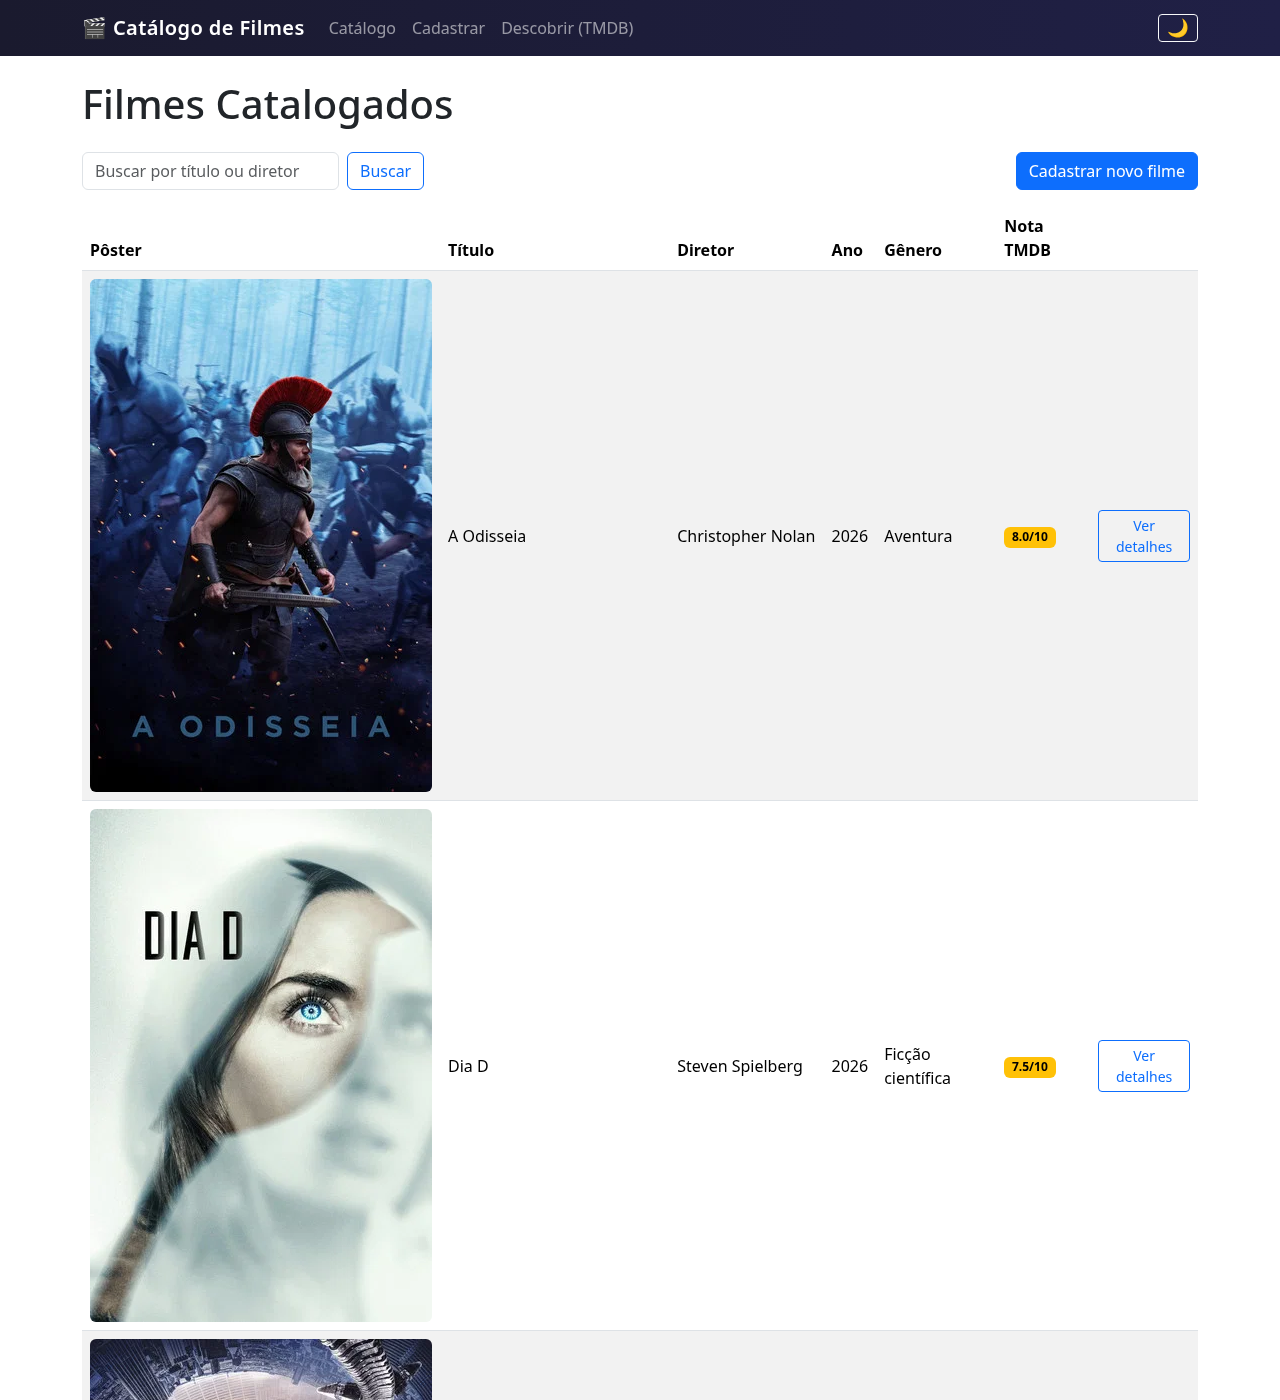
\includegraphics[width=\textwidth]{img/listar-filmes.png}
    \caption{Listagem do catálogo (\texttt{/listarFilmes}).}
    \label{fig:listar}
\end{figure}

\clearpage

\subsection{Cadastro de filme}

O formulário de cadastro (\texttt{/cadastrarFilme}), com o campo obrigatório de título destacado
e o campo opcional de busca por título no TMDB.

\begin{figure}[h!]
    \centering
    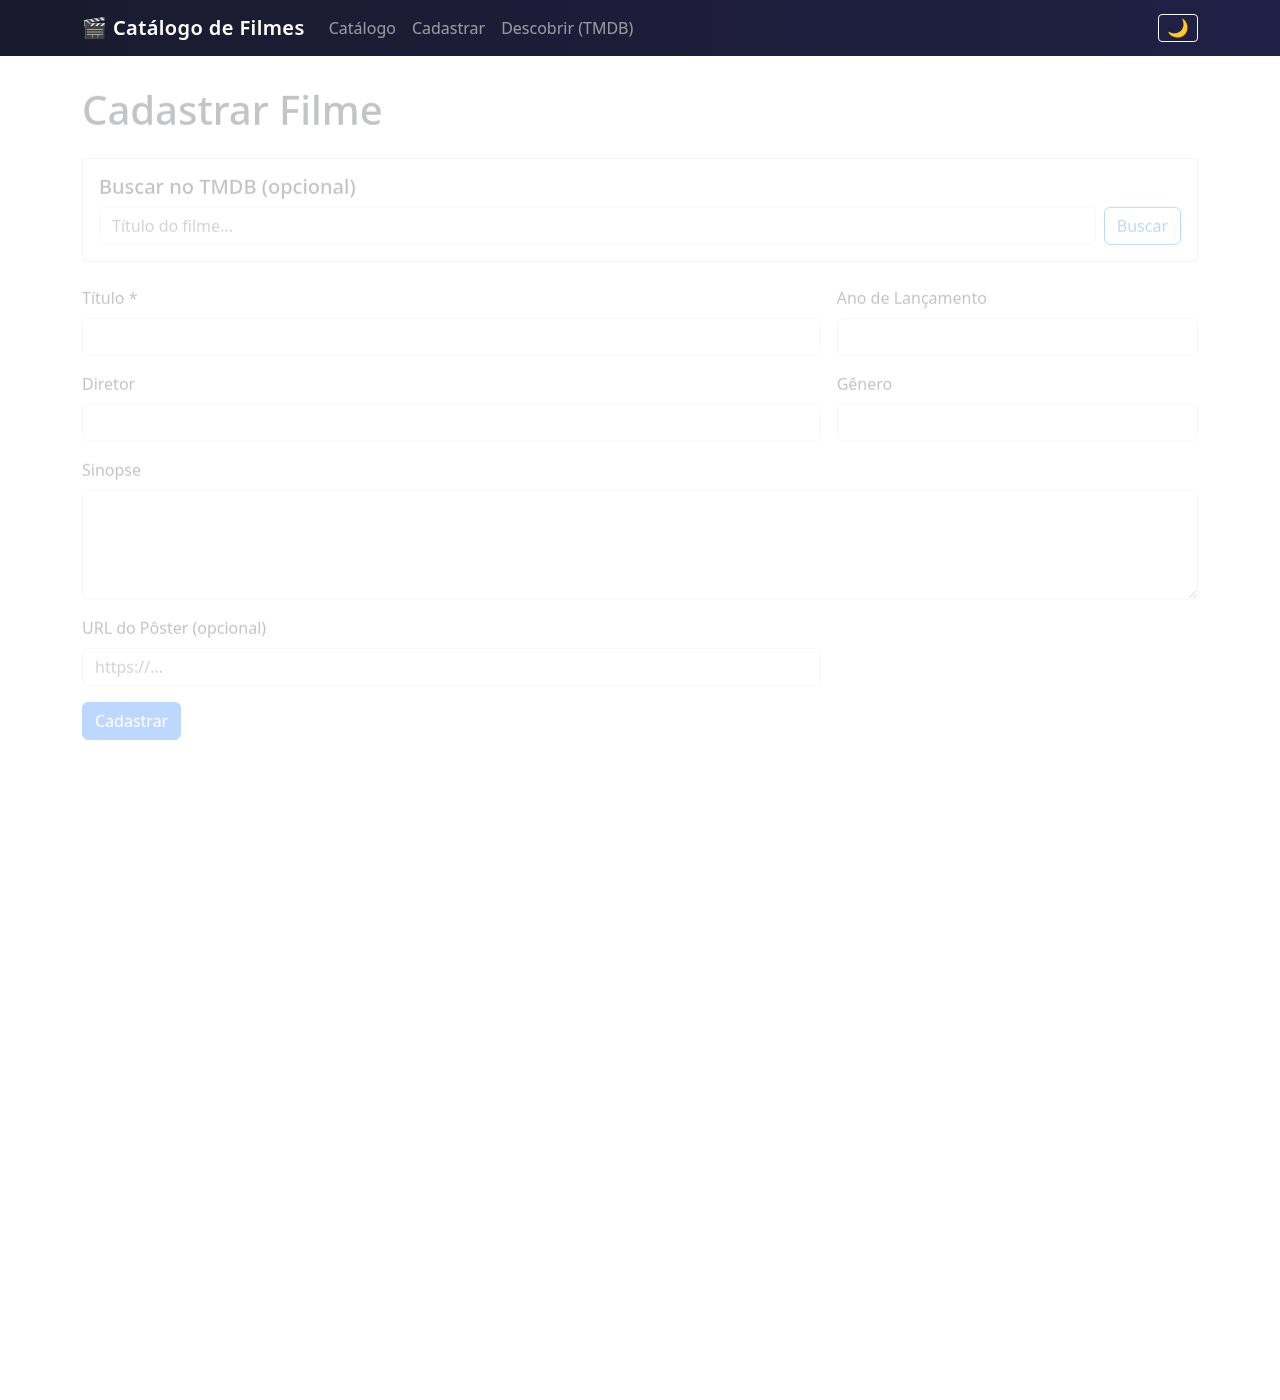
\includegraphics[width=0.85\textwidth]{img/cadastrar-filme.png}
    \caption{Formulário de cadastro (\texttt{/cadastrarFilme}), vazio.}
    \label{fig:cadastrar}
\end{figure}

\subsection{Detalhe de filme}

A página de detalhe (\texttt{/detalharFilme?id=N}) exibe todos os campos de um filme
específico -- no exemplo a seguir, o filme ``A Odisseia'' -- com links para editar e excluir.

\begin{figure}[h!]
    \centering
    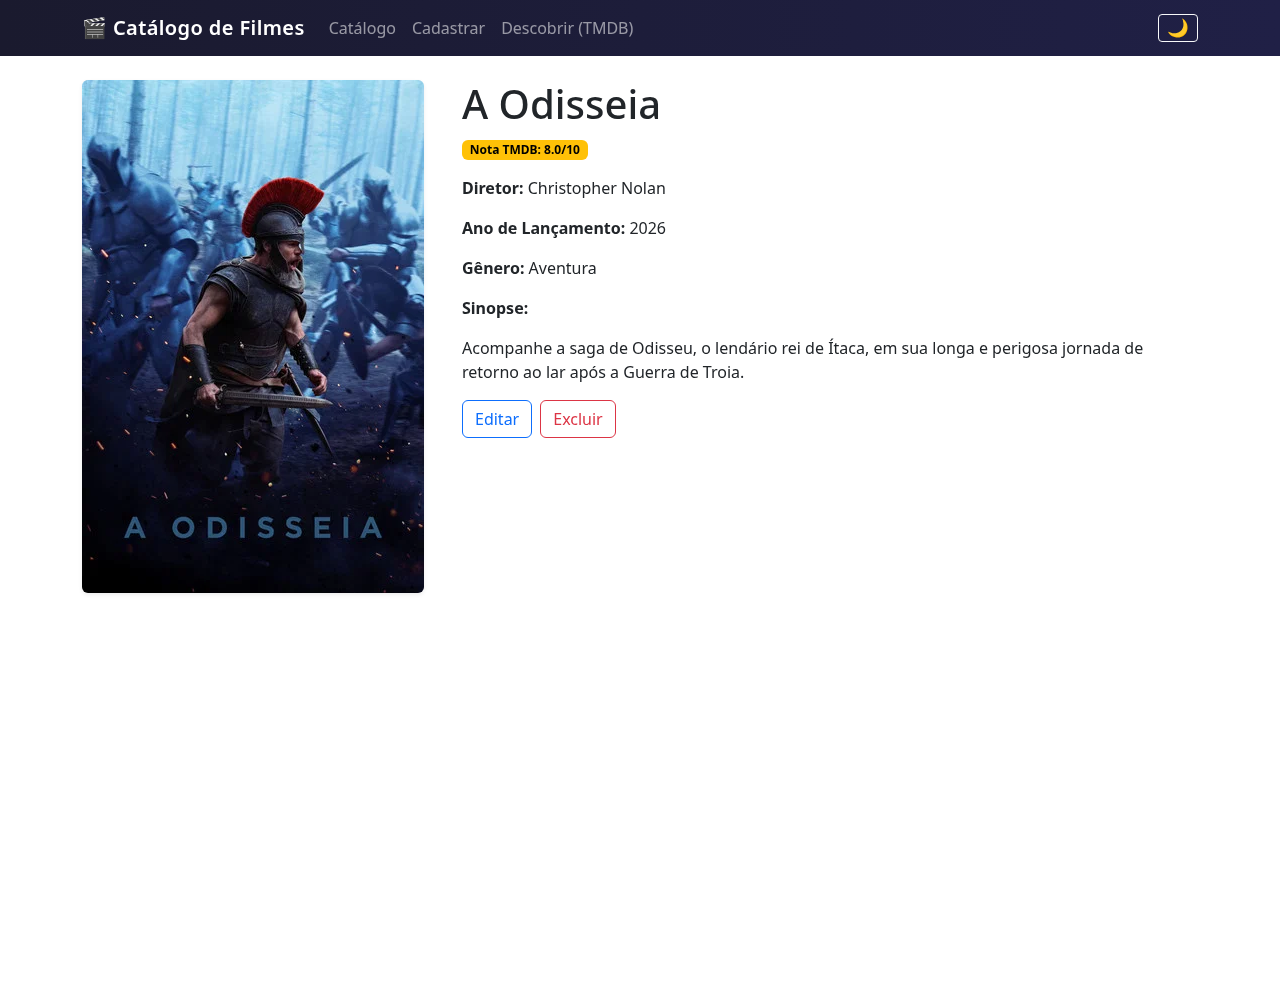
\includegraphics[width=0.85\textwidth]{img/detalhar-filme.png}
    \caption{Página de detalhe de um filme (\texttt{/detalharFilme?id=10}).}
    \label{fig:detalhar}
\end{figure}

\clearpage

\subsection{Edição de filme}

O formulário de edição (\texttt{/editarFilme?id=N}) vem pré-preenchido com os dados atuais do
filme -- no exemplo, ``Tropa de Elite'', já com pôster importado do TMDB visível.

\begin{figure}[h!]
    \centering
    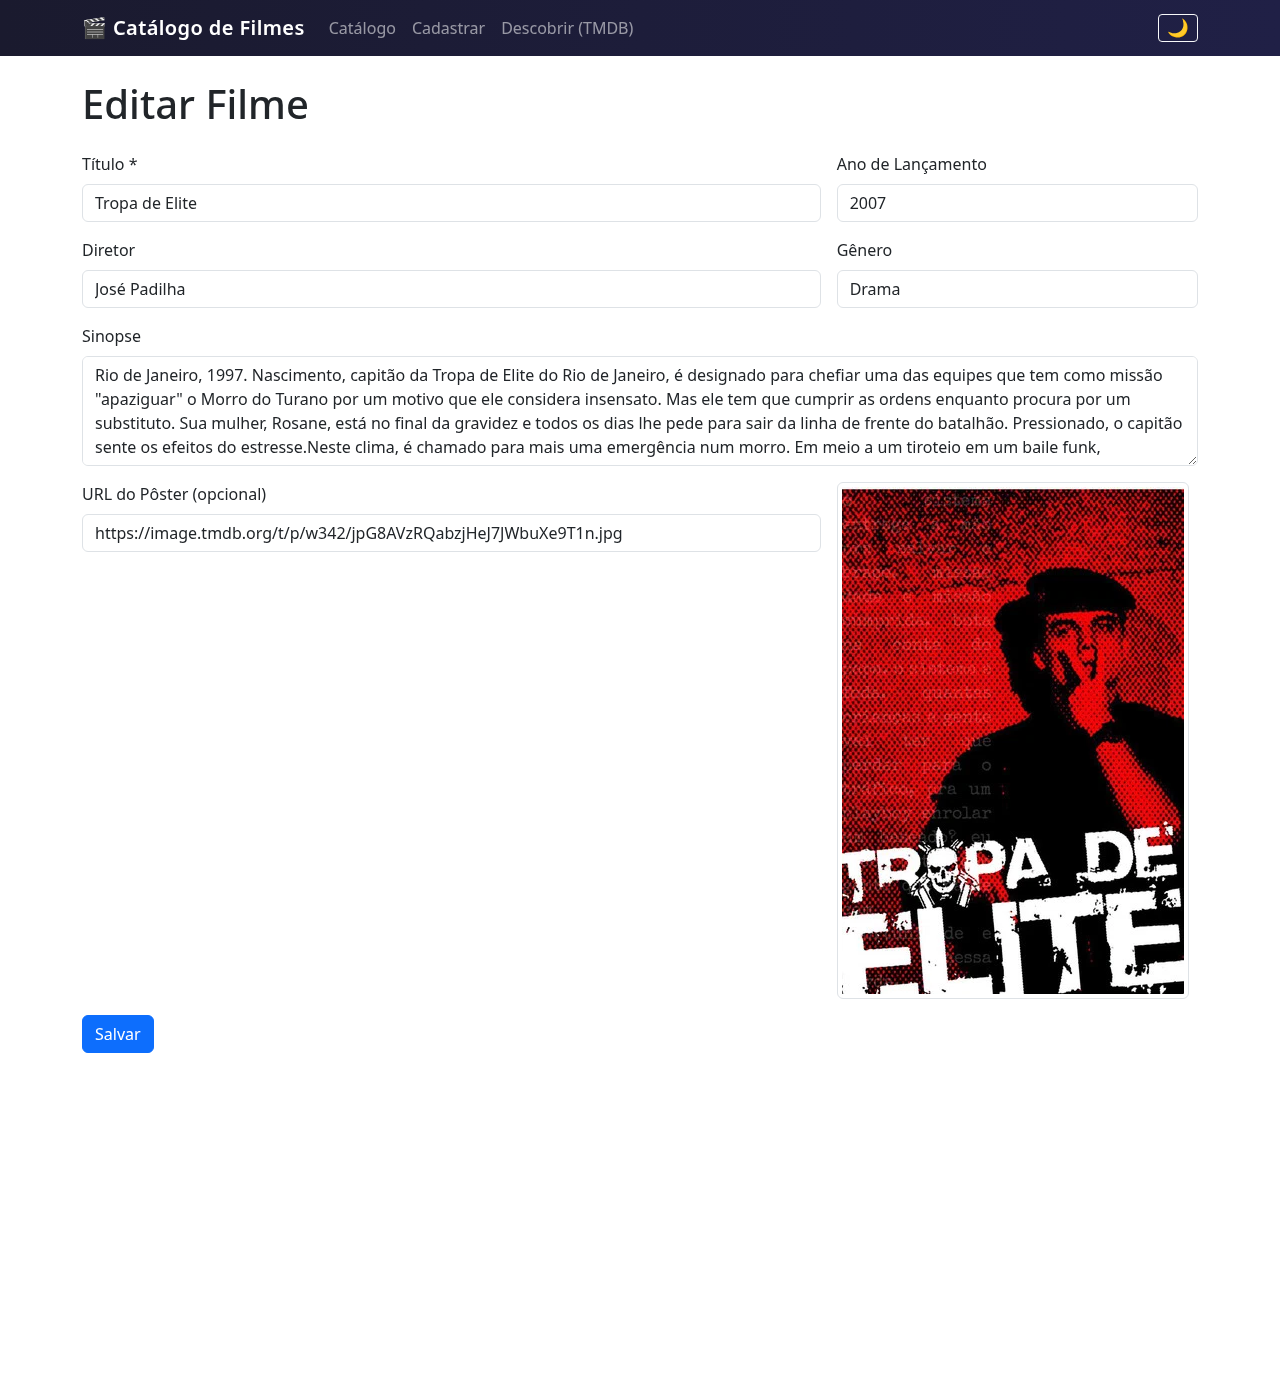
\includegraphics[width=0.85\textwidth]{img/editar-filme.png}
    \caption{Formulário de edição pré-preenchido (\texttt{/editarFilme?id=12}).}
    \label{fig:editar}
\end{figure}

\subsection{Extensão: Descobrir filmes (TMDB)}

O carrossel de filmes populares (\texttt{/descobrirFilmes}), consumindo a API pública do TMDB em
tempo real, com botão de importação direta ao catálogo.

\begin{figure}[h!]
    \centering
    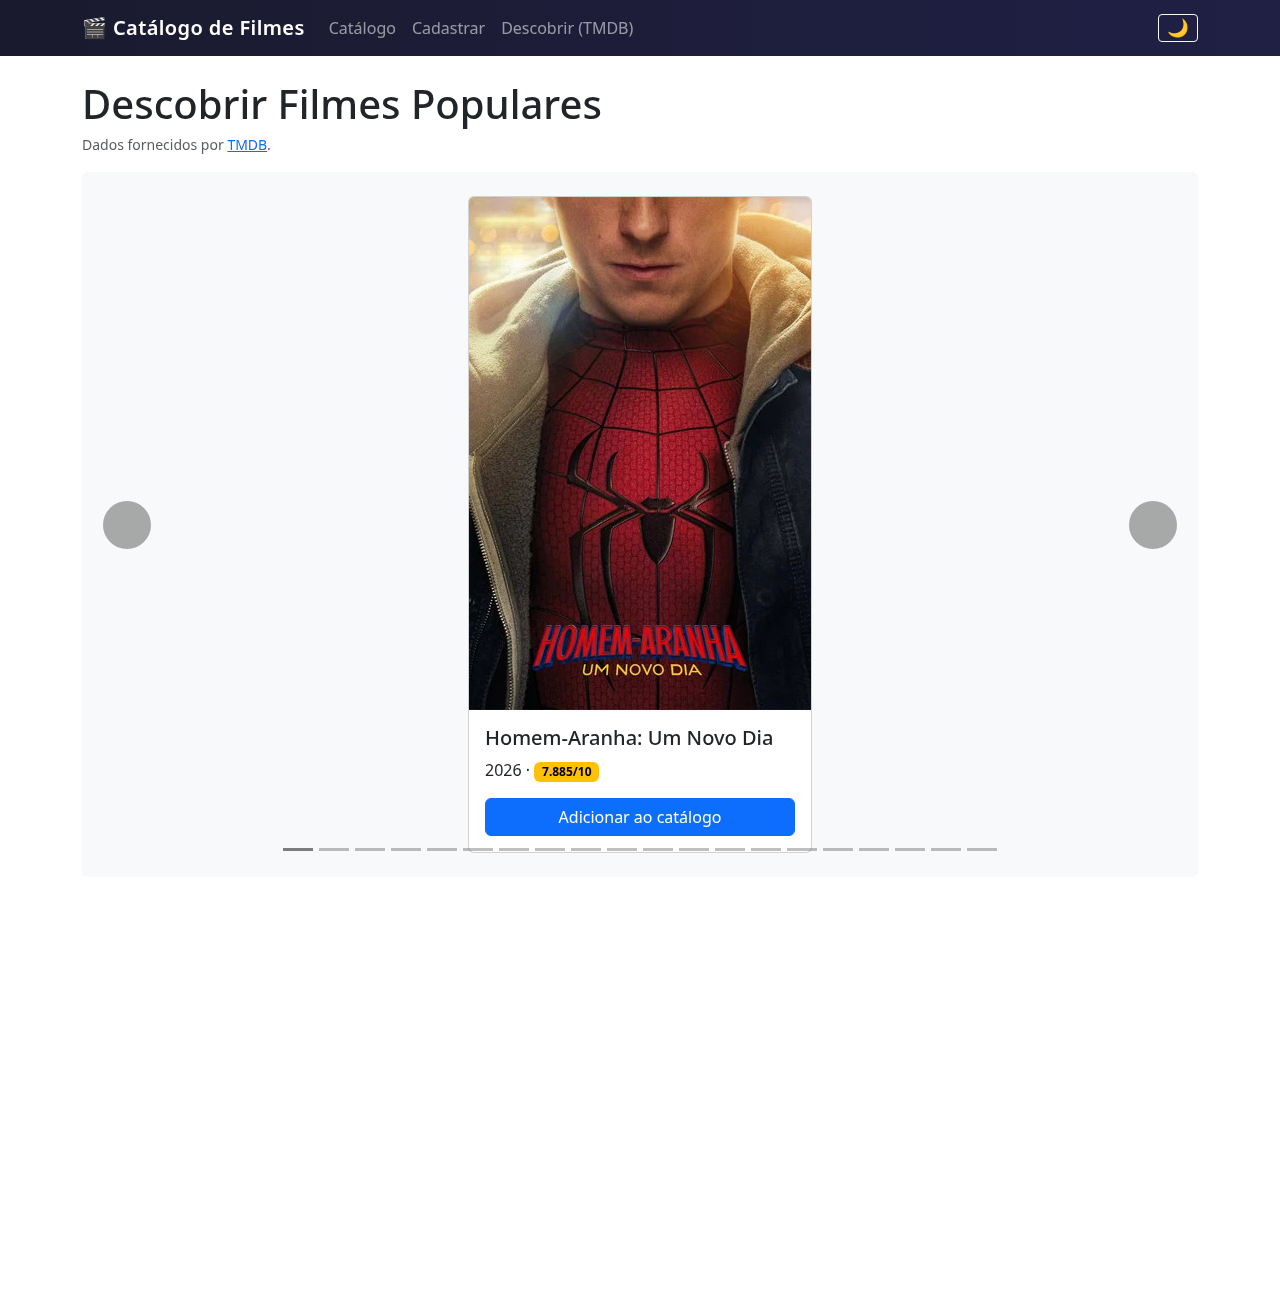
\includegraphics[width=\textwidth]{img/descobrir-filmes.png}
    \caption{Carrossel de filmes populares do TMDB (\texttt{/descobrirFilmes}).}
    \label{fig:descobrir}
\end{figure}

\clearpage

\subsection{Extensão: busca no TMDB dentro do cadastro}

Busca por título consumindo o TMDB diretamente de dentro do formulário de cadastro, exibindo até
cinco resultados para o usuário escolher e pré-preencher o formulário.

\begin{figure}[h!]
    \centering
    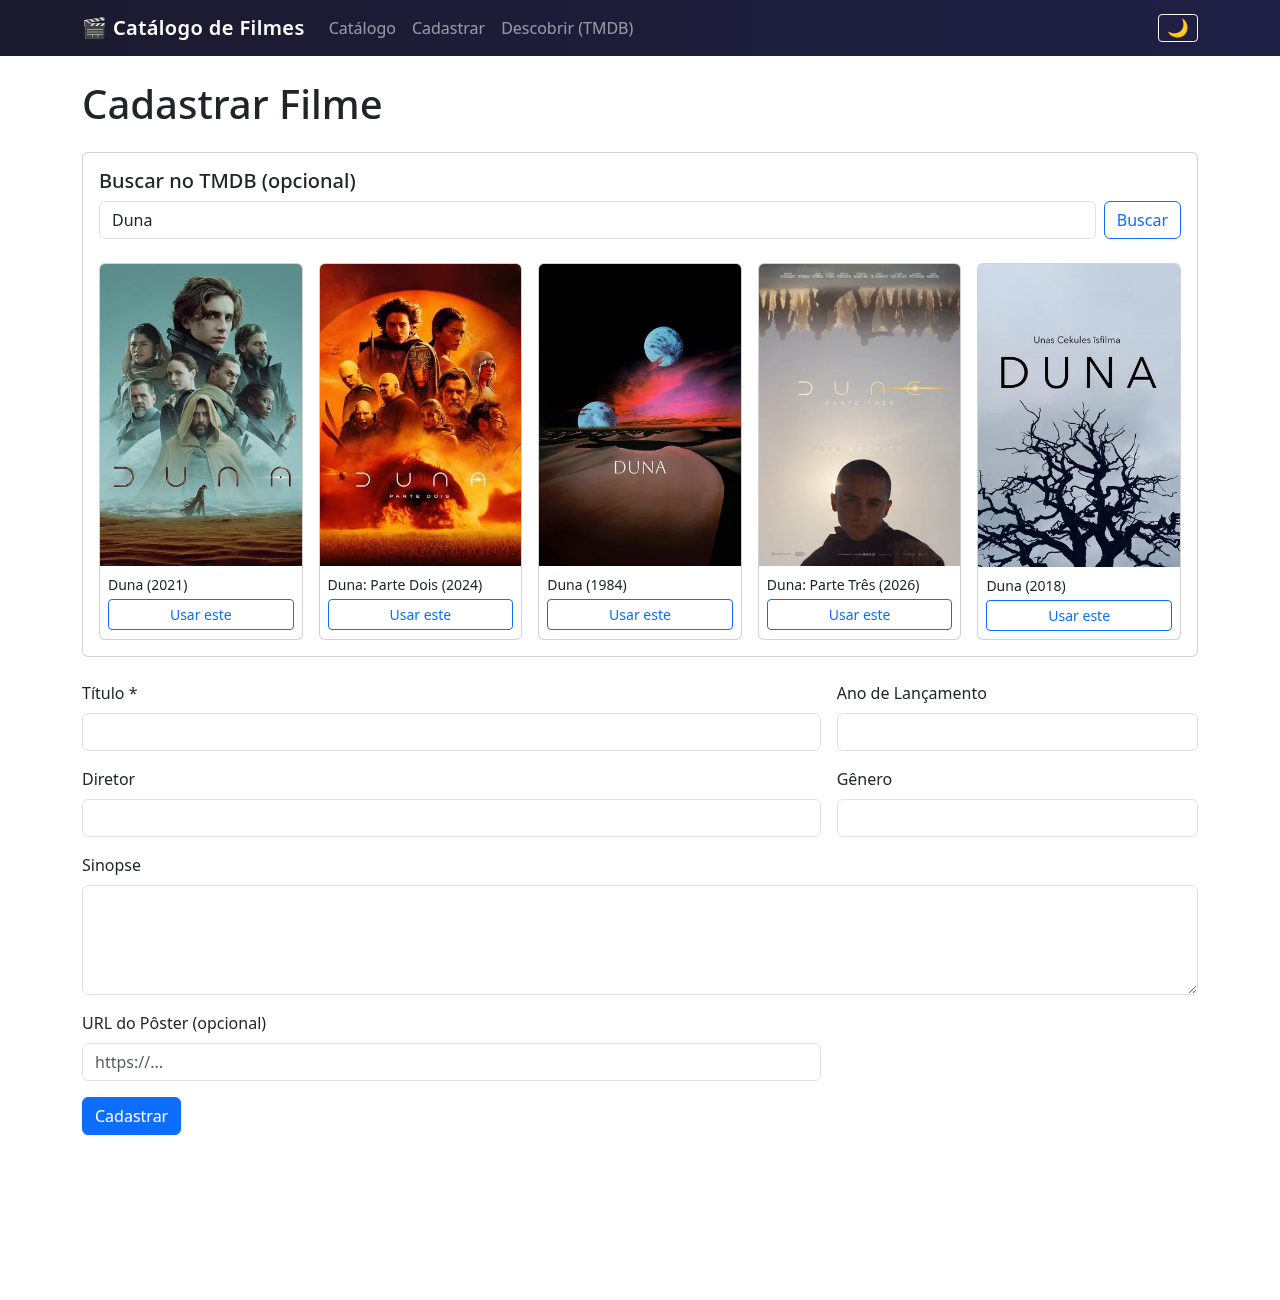
\includegraphics[width=0.85\textwidth]{img/busca-tmdb.png}
    \caption{Busca por título no TMDB, dentro do cadastro (\texttt{/cadastrarFilme?buscaTmdb=Duna}).}
    \label{fig:busca-tmdb}
\end{figure}

% ============================================================================
% 6. CONSIDERAÇÕES SOBRE SEGURANÇA
% ============================================================================
\section{Considerações sobre Segurança}
\label{sec:seguranca}

Tratei a segurança como parte integral do desenvolvimento (princípio de \textit{Secure by
Design}, McGRAW, 2006): apliquei uma revisão de segurança dedicada, seguindo um checklist fixo,
ao final de cada funcionalidade -- \textbf{antes} de qualquer especificação ser considerada
concluída -- e, após a conclusão de todas as funcionalidades mandatórias, executei uma trilha
independente de teste de penetração (\textit{pentest}) \textit{blackbox}, escopada pelo OWASP
Top 10:2021.

\subsection{Revisão de segurança por funcionalidade}

Submeti todas as especificações do projeto (cadastro, listagem, detalhe, edição, exclusão,
busca, integração TMDB e reestilização de interface) a uma revisão de segurança formal, cobrindo
cinco categorias fixas: SQL Injection, tratamento de exceções, validação de dados, XSS
(\textit{Cross-Site Scripting}) e proteção de credenciais/chaves. Os pontos centrais,
consistentes em todo o projeto, são:

\begin{itemize}
    \item \textbf{SQL Injection (situação-problema 1)}: todo acesso ao banco de dados, em
        \texttt{FilmeDAOImpl}, usa \texttt{PreparedStatement} com parâmetros \texttt{?} -- nunca
        concatenação de \textit{string} SQL com entrada do usuário, mesmo dentro de cláusulas
        \texttt{LIKE} (ver Listagem~\ref{lst:busca});
    \item \textbf{Tratamento de exceções (situação-problema 2)}: todo acesso JDBC roda em
        \textit{try-with-resources}; toda \texttt{SQLException} é registrada no log do servidor e
        nunca exposta ao usuário como \textit{stack trace} ou mensagem técnica -- o usuário
        sempre recebe uma mensagem amigável e genérica;
    \item \textbf{Validação de dados}: centralizada em \texttt{FilmeValidator}, aplicada
        \textit{antes} de qualquer persistência -- título obrigatório, ano de lançamento numérico
        quando informado, tamanhos máximos de campo alinhados à DDL da tabela \texttt{filme};
    \item \textbf{XSS}: toda saída de dado originado do usuário (ou do TMDB) nas páginas JSP usa a
        tag JSTL \texttt{<c:out>}, que escapa automaticamente marcação HTML/JavaScript -- nunca
        Expression Language (EL) crua (\texttt{\$\{...\}}) para texto livre de usuário. Isso cobre
        tanto XSS persistente (dados vindos do banco, como na listagem) quanto XSS refletido
        (como o termo de busca reexibido no campo de busca);
    \item \textbf{Credenciais e chaves}: as credenciais de banco de dados (\texttt{db.properties})
        e a chave de API do TMDB (\texttt{tmdb.properties}) nunca são \textit{hardcoded} no
        código-fonte, ficam fora do controle de versão (\texttt{.gitignore}) e são lidas
        exclusivamente por classes utilitárias dedicadas (\texttt{FabricaDeConexoes},
        \texttt{FabricaTmdb}).
\end{itemize}

Obtive aprovação integral em todas as revisões (5/5 itens, com alguns itens marcados
\textit{N/A} quando não aplicáveis, como validação de dados em funcionalidades somente-leitura).
As poucas observações que registrei durante essas revisões classifiquei como não bloqueantes --
lacunas de robustez defensiva, não vulnerabilidades de segurança propriamente ditas (por
exemplo, ausência de validação de faixa de valores em um campo interno que nunca é editado
diretamente pelo usuário) -- e as documentei nas especificações correspondentes para eventual
correção futura.

\subsection{Achados do pentest \textit{blackbox} (Nível 3 -- trilha de segurança)}

Após a conclusão de todas as funcionalidades mandatórias, executei uma trilha independente de
teste de penetração \textit{blackbox}, escopada pelo OWASP Top 10:2021, contra a aplicação em
execução, sob a regra inegociável de \textbf{reportar, nunca explorar}. Registrei dois achados,
ambos já triados e \textbf{encerrados}:

\begin{itemize}
    \item \textbf{Ausência de controle de acesso e de proteção CSRF} (severidade Média,
        OWASP A01:2021 -- \textit{Broken Access Control}). Como a aplicação não implementa
        autenticação -- decisão de escopo consistente com o enunciado, que descreve um catálogo
        de uso pessoal --, qualquer visitante que descubra um \texttt{id} de filme pode, em
        tese, editá-lo ou excluí-lo, e o formulário de exclusão não possui token anti-CSRF (a
        única mitigação é o uso exclusivo de \texttt{POST}, nunca \texttt{GET}, mais uma
        confirmação do lado do cliente). Eu já havia identificado esse indício e o havia
        formalmente aceito como risco durante as revisões de segurança de cada especificação
        individual; o pentest \textit{blackbox} apenas confirmou, de fora, o que eu já sabia.
        Status final: \textbf{Risco Aceito} -- pretendo reavaliar caso implemente uma extensão
        de autenticação no futuro;
    \item \textbf{Ausência de cabeçalhos HTTP de segurança} (severidade Baixa, OWASP A05:2021 --
        \textit{Security Misconfiguration}). A configuração padrão do servidor não incluía
        cabeçalhos de defesa em profundidade como \texttt{X-Frame-Options},
        \texttt{Content-Security-Policy}, \texttt{X-Content-Type-Options} e um atributo
        \texttt{SameSite} explícito no cookie de sessão. Eu \textbf{corrigi} efetivamente este
        achado: implementei um novo filtro de \textit{servlet}, \texttt{CabecalhosSegurancaFilter},
        que adiciona os quatro primeiros cabeçalhos a toda resposta HTTP (com uma
        \textit{Content Security Policy} restrita aos domínios efetivamente usados pela
        aplicação -- CDN do Bootstrap e imagens do TMDB), e configurei o cookie de sessão com
        \texttt{SameSite=Lax} via \texttt{META-INF/context.xml} do Tomcat. Revalidei a correção
        (\texttt{mvn test}, inspeção dos cabeçalhos HTTP reais e confirmação de que nenhuma
        funcionalidade existente foi quebrada). Status final: \textbf{Corrigido}.
\end{itemize}

\subsection{Cobertura de testes}

Escrevi, para a camada de acesso a dados (\texttt{FilmeDAOImpl}), uma suíte de 20 testes JUnit 5
(\texttt{src/test/java/com/catalogo/dao/FilmeDAOTest.java}), que executei de fato (\texttt{mvn
test}) contra um banco MariaDB real, cobrindo todos os métodos de \texttt{FilmeDAO} -- incluindo
casos de sucesso, ausência de correspondência, e um teste específico de sondagem com aspas
simples (\texttt{buscarPorTituloOuDiretor\_naoDeveLancarExcecao\_comAspasSimples}) para
confirmar, empiricamente, a ausência de vulnerabilidade a SQL Injection na funcionalidade de
busca.

% ============================================================================
% 7. CONCLUSÕES
% ============================================================================
\section{Conclusões}

% TODO (autor humano): esta seção é reflexão pessoal e não deve ser gerada
% automaticamente. Preencher com, no mínimo:
%   - Dificuldades encontradas ao longo do desenvolvimento;
%   - Principais aprendizados (técnicos e de processo);
%   - Trabalhos futuros (ex.: autenticação, paginação, filtragem por gênero,
%     testes automatizados de front-end, deploy em produção).
% O texto abaixo é apenas um esqueleto de apoio -- substituir pelo relato real.

\textit{[Preencha esta seção com uma reflexão pessoal, na primeira pessoa, sobre o processo de
desenvolvimento. Sugestão de estrutura: (1) principais dificuldades técnicas que você encontrou;
(2) principais aprendizados, tanto técnicos (Java, Servlets/JSP/JDBC, segurança) quanto de
processo (Aprendizagem Baseada em Projetos, especificação antes de código); (3) possíveis
trabalhos futuros que pretende explorar, por exemplo: implementação de autenticação de usuários
(o que reabriria a discussão de controle de acesso da Seção~\ref{sec:seguranca}), paginação da
listagem, filtragem por gênero, ou testes automatizados end-to-end da camada de apresentação.]}

% ============================================================================
% 8. REFERÊNCIAS
% ============================================================================
\section{Referências}

\subsection{Bibliografia da disciplina}

\begin{itemize}[leftmargin=1.2cm]
    \item BENDER, W. N. \textit{Aprendizagem baseada em projetos}: educação diferenciada para o
        século XXI. 1. ed. Porto Alegre: Penso, 2014.
    \item BLUMENFELD, P. C. et al. Motivating project-based learning: Sustaining the doing,
        supporting the learning. \textit{Educational Psychologist}, [s.l.], v. 26, n. 3-4, p.
        369-398, 1991. Disponível em: \url{https://doi.org/10.1080/00461520.1991.9653139}.
        Acesso em: 05/04/2025.
    \item BOOCH, G.; RUMBAUGH, J.; JACOBSON, I. \textit{UML}: guia do usuário. 2. ed. Rio de
        Janeiro: Elsevier, 2007.
    \item DEITEL, P.; DEITEL, H. \textit{Java\textregistered{}}: como programar. 10. ed. São
        Paulo: Pearson Universidades, 2017.
    \item FOWLER, M. \textit{UML distilled}: a brief guide to the standard object modeling
        language. 3rd ed. Boston: Addison-Wesley Professional, 2004.
    \item INTERNATIONAL ORGANIZATION FOR STANDARDIZATION. \textit{ISO/IEC 27001:2013}:
        Information technology -- Security techniques -- Information security management
        systems -- Requirements. 1st ed. Geneva: ISO, 2013.
    \item KNUTH, D. E. Computer programming as an art. \textit{Communications of the ACM}, v.
        17, n. 12, p. 667-673, Dec. 1974. Disponível em:
        \url{https://doi.org/10.1145/361604.36161}. Acesso em: 05/04/2025.
    \item LARMER, J.; MERGENDOLLER, J.; BOSS, S. \textit{Setting the standard for project-based
        learning}: a proven approach to rigorous classroom instruction. 1st ed. Alexandria:
        ASCD, 2015.
    \item MCGRAW, G. \textit{Software security}: building security in. 1st ed. Upper Saddle
        River: Addison-Wesley, 2006.
    \item MYERS, G. J.; SANDLER, C.; BADGETT, T. \textit{The art of software testing}. 3rd ed.
        Hoboken: John Wiley \& Sons, 2012.
    \item OLIVEIRA, K. Aprendizagem Baseada em Projetos como estratégia para o desenvolvimento de
        atividades não presenciais no ensino médio integrado em informática no IFB Campus
        Brasília. \textit{Revista Brasileira da Educação Profissional e Tecnológica}, v. 2, n.
        22, e11815, 2022 (CC BY 4.0) | ISSN 2447-1801 | DOI:
        \url{https://doi.org/10.15628/rbept.2022.11815}. Acesso em: 05/04/2025.
    \item PRESSMAN, R. S.; MAXIM, B. R. \textit{Engenharia de software}: uma abordagem
        profissional. 8. ed. Porto Alegre: AMGH, 2016.
    \item THOMAS, J. W. \textit{A review of research on project-based learning}. 1st ed. San
        Rafael: Autodesk Foundation, 2000. Disponível em:
        \url{http://www.bobpearlman.org/BestPractices/PBL_Research.pdf}. Acesso em: 25/05/2025.
    \item TRILLING, B.; FADEL, C. \textit{21st century skills}: learning for life in our times.
        1st ed. San Francisco: Jossey-Bass, 2009.
\end{itemize}

\subsection{Documentação técnica consultada}

\begin{itemize}[leftmargin=1.2cm]
    \item ORACLE. \textit{Java Platform, Standard Edition Documentation}. Disponível em:
        \url{https://docs.oracle.com/en/java/javase/}.
    \item ORACLE. \textit{The Java Tutorials -- JDBC Database Access}. Disponível em:
        \url{https://docs.oracle.com/javase/tutorial/jdbc/}.
    \item OWASP FOUNDATION. \textit{OWASP Top 10:2021}. Disponível em:
        \url{https://owasp.org/Top10/}.
    \item THE MOVIE DATABASE (TMDB). \textit{API Documentation}. Disponível em:
        \url{https://developer.themoviedb.org/docs}.
    \item THE BOOTSTRAP AUTHORS. \textit{Bootstrap 5 Documentation}. Disponível em:
        \url{https://getbootstrap.com/docs/5.3/}.
    \item ORACLE. \textit{How to Write Doc Comments for the Javadoc Tool}. Disponível em:
        \url{https://www.oracle.com/technical-resources/articles/java/javadoc-tool.html}.
\end{itemize}

% ============================================================================
% 9. DOCUMENTAÇÃO DO CÓDIGO-FONTE
% ============================================================================
\section{Documentação do Código-Fonte}

Comentei todo o código-fonte Java do projeto de duas formas complementares. Primeiro,
comentários de linha (\texttt{//}) explicam decisões de design pontuais e blocos de lógica não
óbvia diretamente no ponto onde ocorrem -- por exemplo, a razão pela qual o filtro de codificação
UTF-8 precisa ser o primeiro da cadeia de filtros, ou por que o campo \texttt{notaTmdb} é do tipo
\texttt{Double} (objeto) em vez de \texttt{double} (primitivo). Segundo, e mais formalmente, toda
classe pública e todo método público de \texttt{com.catalogo.dao}, \texttt{com.catalogo.servlet}
e \texttt{com.catalogo.service} possuem comentários \textbf{Javadoc} (\texttt{/** ... */}),
seguindo a convenção padrão da linguagem Java, incluindo descrição do propósito, parâmetros
(\texttt{@param}), retorno (\texttt{@return}) e exceções lançadas (\texttt{@throws}) quando
aplicável.

A interface \texttt{FilmeDAO} e a classe \texttt{FabricaDeConexoes} já continham Javadoc completo
desde a implementação original de cada funcionalidade. Nesta rodada final de documentação,
auditei e complementei o Javadoc nos métodos \texttt{doGet}/\texttt{doPost} de todos os sete
Servlets do projeto e no método \texttt{doFilter} dos dois filtros de \textit{servlet}
(\texttt{CodificacaoUtf8Filter} e \texttt{CabecalhosSegurancaFilter}), que já possuíam Javadoc a
nível de classe, mas ainda não a nível de método -- nove classes ao todo passaram a ter Javadoc
de método, descrevendo especificamente a rota/operação HTTP tratada por cada uma, seus
parâmetros de requisição e o comportamento em caso de erro. No Javadoc de
\texttt{com.catalogo.model.Filme}, segui a recomendação da disciplina de manter um comentário de
classe curto (sem Javadoc redundante em cada \textit{getter}/\textit{setter} trivial).

% ============================================================================
% 10. MANUAL DO USUÁRIO SIMPLIFICADO
% ============================================================================
\section{Manual do Usuário Simplificado}

Escrevi um manual do usuário simplificado, voltado a quem nunca utilizou o sistema (linguagem
não técnica), disponível separadamente em \texttt{docs/manual-usuario.md}. Ele cobre, em uma a
duas páginas, como acessar a aplicação, cadastrar um novo filme (incluindo o uso opcional da
busca por título no TMDB), listar e buscar filmes já cadastrados, visualizar os detalhes de um
filme, editá-lo e excluí-lo, além de uma breve seção de dúvidas frequentes -- entre elas, por que
o sistema não exige login (decisão de escopo já discutida na Seção~\ref{sec:seguranca} deste
relatório).

\end{document}
